\documentclass[border=10pt]{standalone}
\usepackage{amsmath,amssymb}
\usepackage{tikz}
\usetikzlibrary{arrows.meta,positioning}
\definecolor{srccol}{RGB}{37,99,235}
\definecolor{relcol}{RGB}{217,119,6}
\definecolor{rxcol}{RGB}{5,150,105}
\definecolor{boxcol}{RGB}{241,245,249}
\newcommand{\herm}{^{H}}
\begin{document}
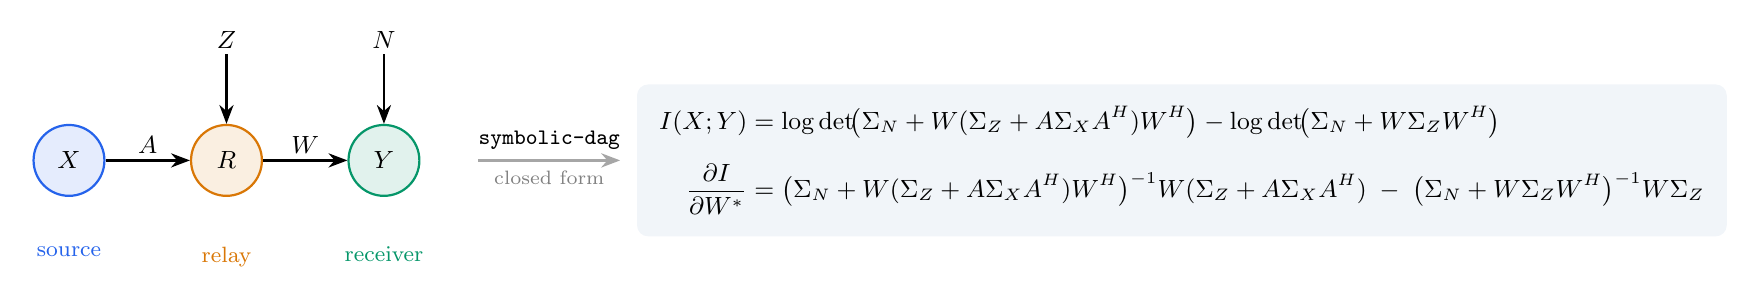
\begin{tikzpicture}[
  >={Stealth[length=2.4mm]}, thick, font=\small,
  src/.style={circle,draw=srccol,fill=srccol!12,minimum size=9mm,inner sep=0pt},
  rel/.style={circle,draw=relcol,fill=relcol!12,minimum size=9mm,inner sep=0pt},
  rx/.style ={circle,draw=rxcol,fill=rxcol!12,minimum size=9mm,inner sep=0pt},
]
% --- two-hop amplify-and-forward relay (a linear Gaussian DAG) ---
\node[src] (x) at (0,0)   {$X$};
\node[rel] (r) at (2.0,0) {$R$};
\node[rx]  (y) at (4.0,0) {$Y$};
\draw[->] (x) -- node[above,inner sep=2pt]{$A$} (r);
\draw[->] (r) -- node[above,inner sep=2pt]{$W$} (y);
\draw[->] (2.0,1.35) node[above,inner sep=1.5pt]{$Z$} -- (r);
\draw[->] (4.0,1.35) node[above,inner sep=1.5pt]{$N$} -- (y);
\node[srccol,font=\footnotesize,below=5mm of x] {source};
\node[relcol,font=\footnotesize,below=5mm of r] {relay};
\node[rxcol, font=\footnotesize,below=5mm of y] {receiver};

% --- engine arrow ---
\draw[->,line width=1.1pt,gray!70] (5.2,0) -- (7.0,0)
  node[midway,above,black,font=\footnotesize\ttfamily]{symbolic-dag}
  node[midway,below,gray,font=\scriptsize]{closed form};

% --- closed form (algebraically reduced library output, machine-verified) ---
\node[anchor=west,align=left,fill=boxcol,rounded corners=4pt,inner sep=8pt] at (7.2,0) {%
$\displaystyle
\begin{aligned}
I(X;Y) &= \log\det\!\bigl(\Sigma_N + W(\Sigma_Z + A\Sigma_X A\herm)W\herm\bigr)
         - \log\det\!\bigl(\Sigma_N + W\Sigma_Z W\herm\bigr) \\[5pt]
\frac{\partial I}{\partial W^{*}} &=
   \bigl(\Sigma_N + W(\Sigma_Z + A\Sigma_X A\herm)W\herm\bigr)^{-1} W(\Sigma_Z + A\Sigma_X A\herm)
   \;-\; \bigl(\Sigma_N + W\Sigma_Z W\herm\bigr)^{-1} W\Sigma_Z
\end{aligned}$};
\end{tikzpicture}
\end{document}
